% Chapter 1

\chapter{Introducción general} % Main chapter title

\label{Chapter1} % For referencing the chapter elsewhere, use \ref{Chapter1} 
\label{IntroGeneral}

%----------------------------------------------------------------------------------------

% Define some commands to keep the formatting separated from the content 
\newcommand{\keyword}[1]{\textbf{#1}}
\newcommand{\tabhead}[1]{\textbf{#1}}
\newcommand{\code}[1]{\texttt{#1}}
\newcommand{\file}[1]{\texttt{\bfseries#1}}
\newcommand{\option}[1]{\texttt{\itshape#1}}
\newcommand{\grados}{$^{\circ}$}

%----------------------------------------------------------------------------------------

%\section{Introducción}

%----------------------------------------------------------------------------------------
\section{El espacio como recurso estratégico}
\label{sec:invap}

\begin{figure}[htbp]
	\centering
	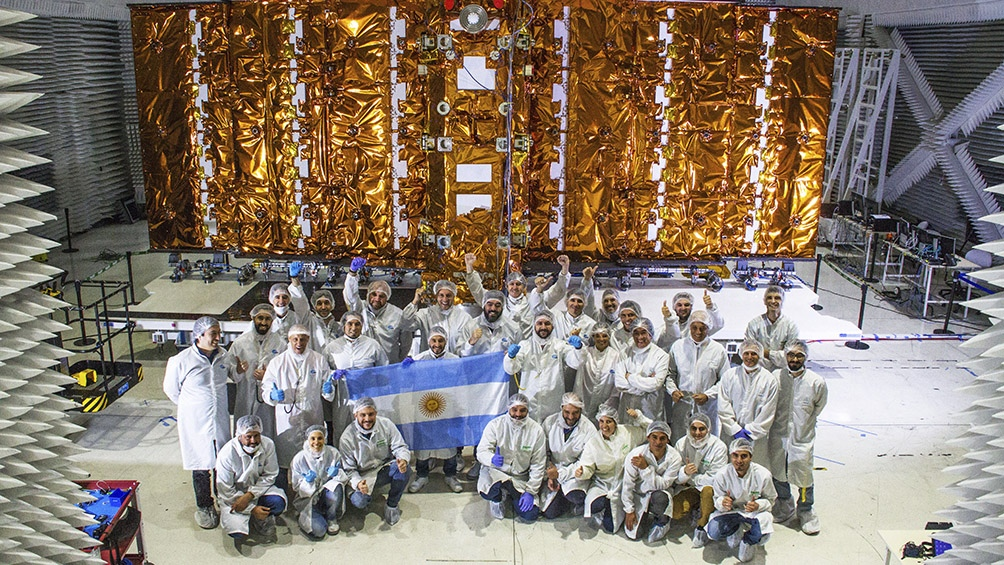
\includegraphics[width=.8\textwidth]{./Figures/invapsaocom.jpg}
	\caption{Satélite SAOCOM\citep{WEBSITE:invap}.}
	\label{fig:saocom}
\end{figure}

\section{Radiación cósmica y sus efectos}
\label{sec:radiacion}

\begin{figure}[htbp]
	\centering
	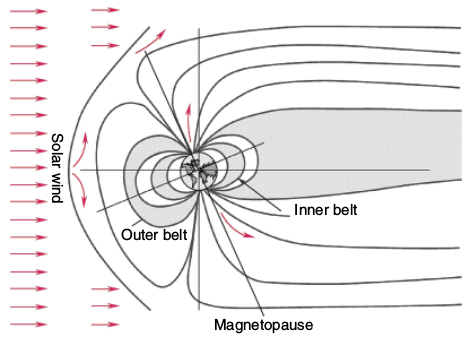
\includegraphics[width=.8\textwidth]{./Figures/vientosolar.jpg}
    \caption{Capas magnéticas de la tierra y viento solar\citep{WEBSITE:structure_space_radiation}.}
	\label{fig:viento}
\end{figure}

\begin{table}[h]
	\centering
	\caption[Efectos de la radiación cósmica]{Efectos producidos por la radiación cósmica\citep{WEBSITE:structure_space_radiation}}
	\begin{tabular}{l c c}    
		\toprule
		\textbf{Evento}      & \textbf{Acrónimo} & \textbf{Efecto}\\
		\midrule
		Latch-up             & SEL               & Pico de corriente\\		
		Upset                & SEU               & Alteración de datos\\
		Funtional Interrupt  & SEFI              & Cambios en la configuración\\
		Transient            & SET               & Pico de tensión\\
		Burnout              & SEB               & Activación de transistores parásitos\\
		Gate Rapture         & SEGR              & Generación de plasma de alta densidad\\
		\bottomrule
		\hline
	\end{tabular}
	\label{tab:radiacion}
\end{table}

\begin{figure}[htbp]
	\centering
	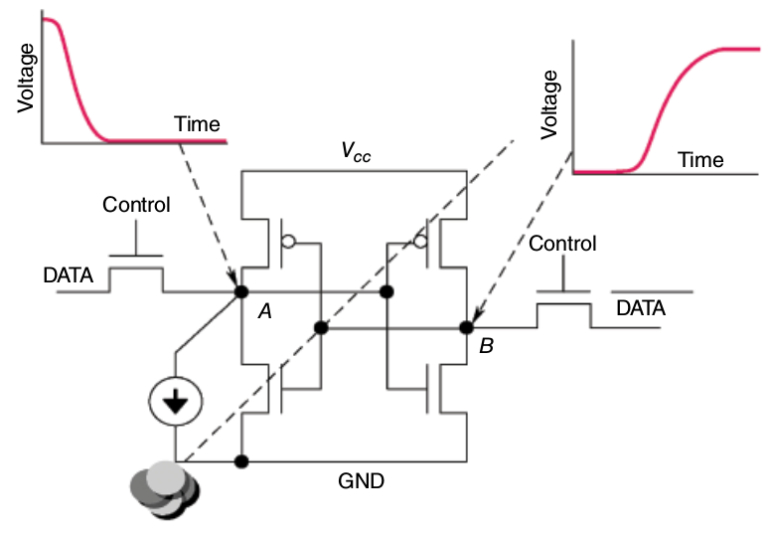
\includegraphics[width=.8\textwidth]{./Figures/bitflip.jpg}
    \caption{Ejemplo simplificado de \emph{bit flip} en un bloque \emph{SDRAM}\citep{WEBSITE:effects_on_devices}.}
	\label{fig:bitflip}
\end{figure}

\begin{table}[h]
	\centering
	\caption[Cinturón de Van Allen]{Cinturón de Van Allen\citep{WEBSITE:structure_space_radiation}}
	\begin{tabular}{l c c}    
		\toprule
		\textbf{Cinturon} & \textbf{Frontera}           & \textbf{Partícula dominante}\\
		\midrule
		Interior          & 1.2 - 2.5 radios terrestres & Protones de alta energía\\		
		Exterior          & 2.8 - 12 radios terrestres  & Electrónes de alta energía\\
		\bottomrule
		\hline
	\end{tabular}
	\label{tab:capasmagneticas}
\end{table}

\section{Calificación espacial e iniciativa \emph{new space}}
\label{sec:newspace}

\begin{figure}[htbp]
	\centering
	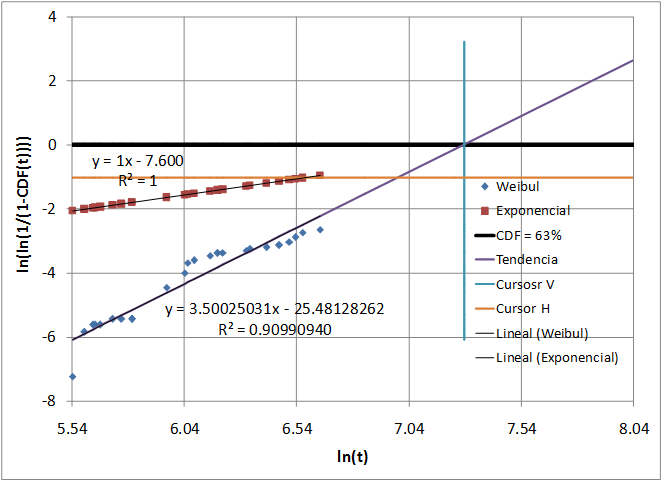
\includegraphics[width=.8\textwidth]{./Figures/starlinkdeath.png}
    \caption{Gráfico Weibull de expectativa de vida \emph{Starlink}\citep{ARTICLE:cibils}.}
	\label{fig:starlinkdeath}
\end{figure}

\begin{figure}[htbp]
	\centering
	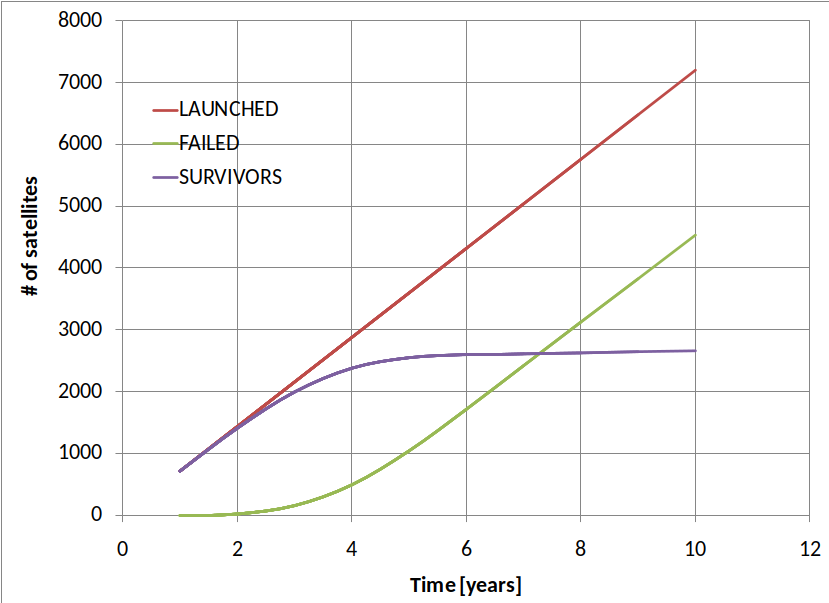
\includegraphics[width=.8\textwidth]{./Figures/starlinkpopulation.png}
    \caption{Proyección de la constelación \emph{Starlink}\citep{ARTICLE:cibils}.}
	\label{fig:starlinkdeath}
\end{figure}

\begin{table}[h]
	\centering
    \caption[Proyección de \emph{debris}]{Proyección de \emph{debris} de \emph{Starlink}\citep{ARTICLE:cibils}}
	\begin{tabular}{c c c c c}    
		\toprule
        \textbf{Lanzamientos} & \textbf{Satélites} & \textbf{Total lanzados} & \textbf{Población} & \textbf{Debris}\\
		\midrule
        12                    & 60                 & 7200                    & 2704               & 4046\\		
        12                    & 180                & 21600                   & 8105               & 12146\\		
        12                    & 400                & 48000                   & 18007              & 26994\\		
        180                   & 60                 & 108000                  & 40000              & 61200\\		
        60                    & 180                & 108000                  & 40000              & 61200\\		
        27                    & 400                & 108000                  & 40000              & 61200\\		
		\bottomrule
		\hline
	\end{tabular}
	\label{tab:starlinkdebris}
\end{table}

\section{Estado del arte}
\label{sec:arte}

\begin{figure}[htbp]
	\centering
	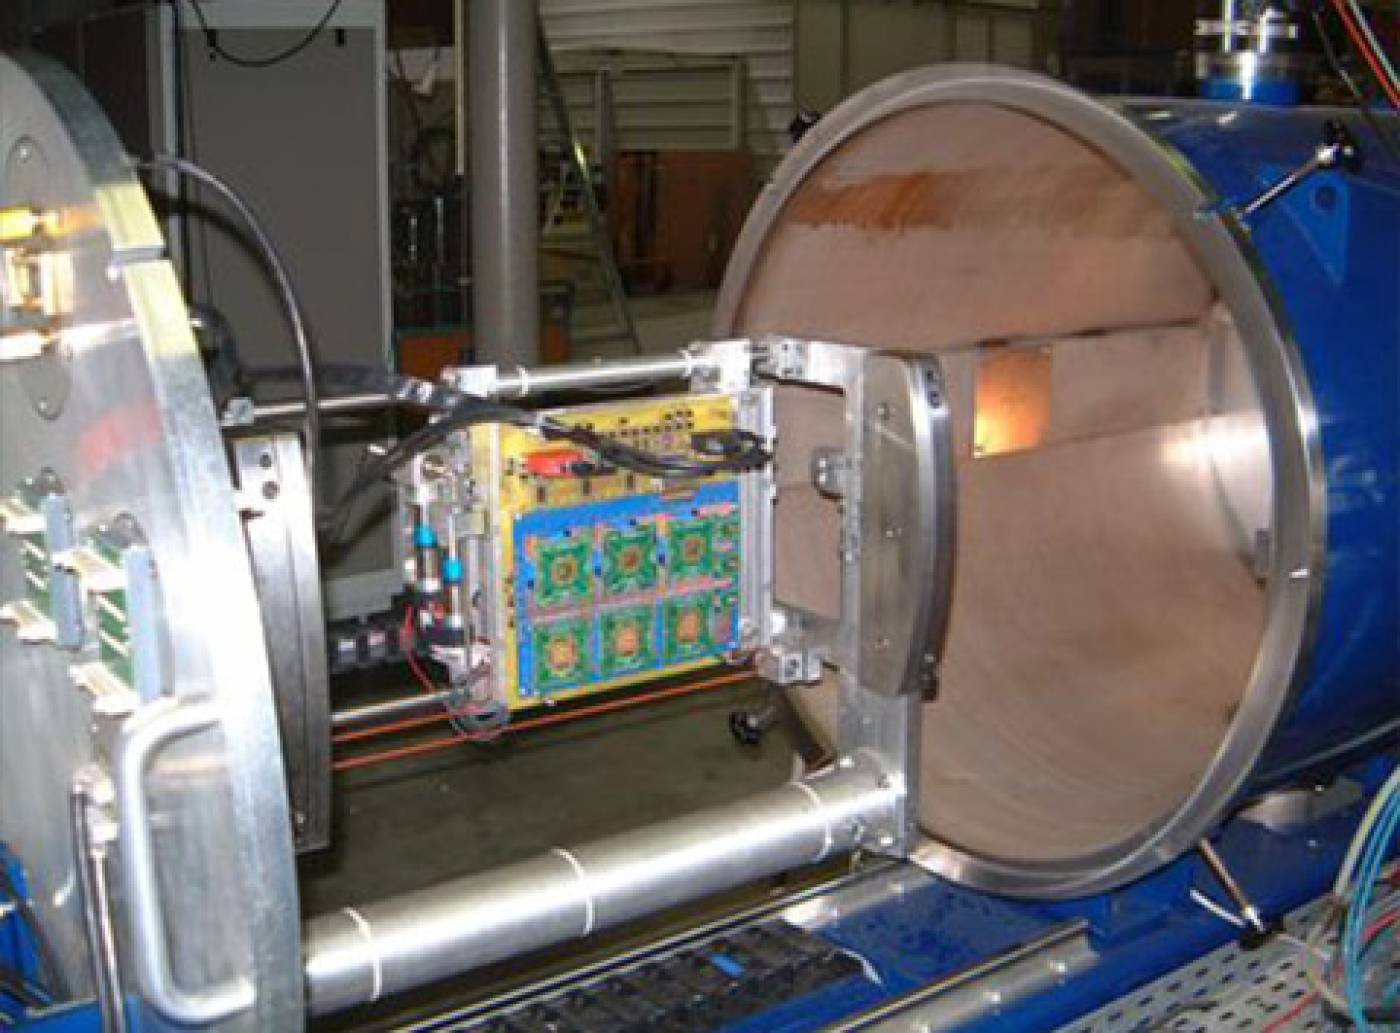
\includegraphics[width=.8\textwidth]{./Figures/heavy_ion_latchup_tests_in_louvain_la_neuve.jpg}
    \caption{Cámara de pruebas de iones pesados\citep{WEBSITE:heavy_ion}.}
	\label{fig:iones}
\end{figure}

\begin{table}[h]
	\centering
	\caption[Comparación de métodos de simulación]{Comparación de métodos de simulación\citep{ARTICLE:velazco}}
	\begin{tabular}{l c c c}    
		\toprule
        \textbf{Método} & \textbf{Eficiencia} & \textbf{Costo} & \textbf{Limitación}\\
		\midrule
        Software        & Baja                & Bajo           & Ciclos de CPU\\		
        Hardware        & Media               & Medio          & Acceso al integrado\\
        Radiación       & Alta                & Alto           & Control del ensayo\\
		\bottomrule
		\hline
	\end{tabular}
	\label{tab:arte}
\end{table}

\section{Alcance del trabajo}

\begin{figure}[htbp]
	\centering
	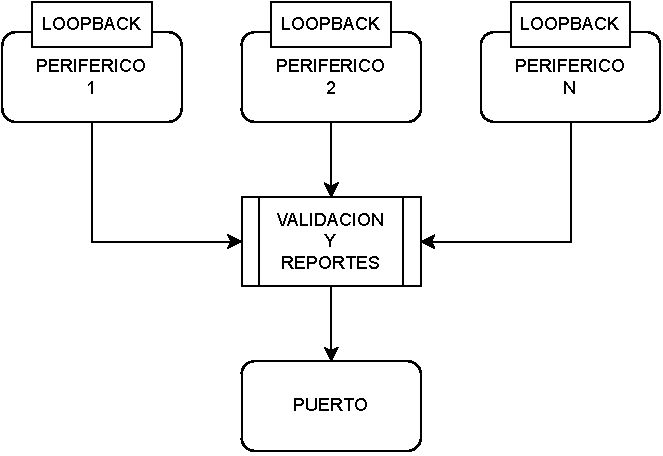
\includegraphics[width=.8\textwidth]{./Figures/dutsimple.pdf}
    \caption{Diagrama simplificado del dispositivo bajo prueba.}
	\label{fig:dutsimple}
\end{figure}

\begin{figure}[htbp]
	\centering
	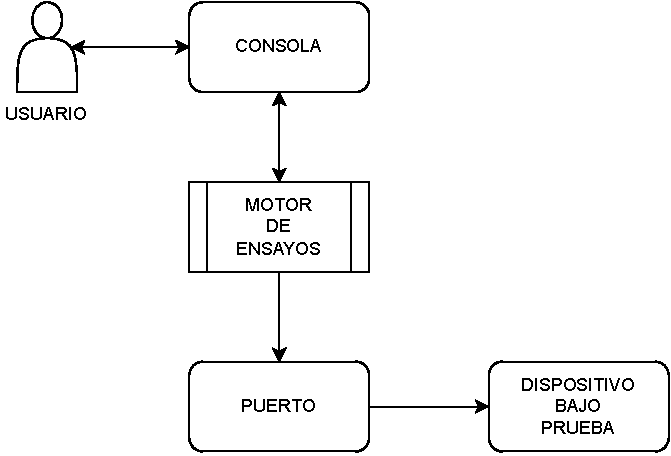
\includegraphics[width=.8\textwidth]{./Figures/sisesimple.pdf}
    \caption{Diagrama simplificado del sistema de inyección de errores.}
	\label{fig:sisesimple}
\end{figure}

\label{sec:alcance}
